\section{TRI-D Interferometric imaging}\seclab{Intf}

Interferometry can be performed working only with the signals measured in the antennas, i.e.\ without unfolding the antenna function, and is referred to as Signal Interferometry (SI), which is by now considered obsolete. This because the method has many unsolved issues with signs due to the antenna function and the emission pattern being angle dependent. More sophisticated is to convert the measured signal in the X- and Y- dipoles to the radiation electric field at the antenna and use this for interferometry, presently the preferred and only option. This will be named E-field Interferometry (EI) when it needs to be contrasted with SI.

Source finding is performed by the script \verb!"Interferometry.sh"! residing in the FlashFolder. The running of the script is controlled by \verb!"Interferometry.in"!, which typically resembles:

\begin{linenumbers}
\resetlinenumber
\tiny
\begin{verbatim}
 &Parameters  RunOption= "TRI-D"
 OutFileLabel= "XYZ"
 AntennaRange= 100.     ! Maximum distance (from the core) for the range of the antennas (in [km]).
 TimeBase=320.    ! Time-offset from the start of the data, best if kept the same for all analyses for this flash
! Simulation= ""     ! Run on simulated data from such files.
! ChainRun= 0     ! Automatically start jobs (for - previous or + following timeslots, made to follow a negative leader.
! IntfSmoothWin= 19     ! Width (in samples) of the slices for TRI-D imaging.
! PixPowOpt= 0     ! =0=default: Intensity=sum two transverse polarizations only; =1: Intensity=sum all polarizations weighted with alpha == intensity of F vector; =2: Intensity=sum all three polarizations, including longitudinal with the full weight
! CalibratedOnly= T     ! Use only antennas that have been calibrated.
 NoiseLevel= 1.0000000000000000E-002     ! Any weaker sources will not be imaged.
 Calibrations="Calibrations202202071332.dat" ! FldCal all antennas
 BadAnt_SAI=   5095,   7093,  11089,  13088,  13089,  17084,  17085,  17094,  17095
               101085, 141083, 141086, 141087, 167094, 169082, 169090, 169094,
 ExcludedStat=  "RS305"      ! Mnemonics of the stations that should be excluded.
 SignFlp_SAI=  142092, 142093
 SaturatedSamplesMax= 3     ! Maximum number of saturates time-samples per chunk of data
 &end  !
S  231.  8.2 ,-3.7, -34.11    !    Reference/Source-| time, & position
C   80 2.5, 30 2.5, 72 4 !   Polar(Phi,Th,R)/Carthesian(N,E,h) | 3x(#gridpoints, grid spacing)
F  25000  15000 10.   !  First/Median| SumStrt, SumWindw, AmpltPlot
\end{verbatim}
\end{linenumbers}

The lines in the namelist \verb!"&Parameters"! input specify:
\begin{enumerate*}
\item \verb!RunOption= "TRI-D"!: Run the TRI-D Imager
\item \verb!OutFileLabel="XYZ"!: Additional label used for the output files, including the plots.
\item \verb!AntennaRange=100.!: The maximal distance (in [km]) from the reference station of the antenna stations that are included in imaging.
\item \verb!TimeBase=320.!: This time is added to the relative time specified in the input.
\item \verb# Simulation= ""#: No simulated data are used in blank, otherwise the simulated data are read from these files and should have the same value as used when generating the simulated data, see \secref{Sim}.
\item \verb# ChainRun=0# (Integer, default=0): If =0 the present run will not spawn any children, otherwise see \secref{ChainRun}.
\item \verb!IntfSmoothWin=19! (Integer, default=20): the width of the sampling function used for Time Resolved Imaging (in [samples]). This number should be of the order of the impulse-response time, about 20~samples.
\item \verb!PixPowOpt=! (Integer, 0): selects how the intensity of a pixel is calcula
   \\\verb!PixPowOpt =0! (default): sum two transverse (as seen from the core) polarizations only.
   \\\verb!PixPowOpt =1! : sum all polarizations weighted with alpha to compensate $A^{-1}$ thus intensity =  $|\vec{F}|$, see \eqref{F_as}.
   \\\verb!PixPowOpt =2! : Sum all three polarizations, thus including longitudinal with the full weight.
\item \verb!CalibratedOnly= T! (logical, .true.): use only antennas that have been calibrated.
\item \verb!NoiseLevel=!: only sources with a coherent intensity exceeding this value will be imaged.
\item \verb!Calibrations =""!: The name of the file containing calibration data.
\item \verb!"BadAnt_SAI="!: These antennas are excluded from the analysis.
\item \verb!"SignFlp_SAI="!: The amplitude for this antenna is multiplied by minus unity.
\item \verb!"ExcludedStat="!: Mnemonics of the stations that will be excluded from interferometry. The exclusion is usually based on unexpected phases.
\end{enumerate*}


The following lines specify:
\begin{enumerate*}
\item[line +1:]   ``\verb#S  231.  8.2 ,-3.7, -34.11#''
   \begin{enumerate*}
   \item[1] Option, "R" or "S" (capital, the very first character on this line): time is specified at the Reference antenna or at the Source location for the tesseract.
   \item[2] $t_t$, the starting time of the data-chunk in which the tesseract is taken, given in time [ms]. Time is taken relative to \verb!"TimeBase"!.
   \item[3-5] Space coordinates of the center of this tesseract, in (N,E,h) notation. The units may be [km] or in [m], but have to be the same for all three.
   \end{enumerate*}
\item[line +2:]   ``\verb#C   80 2.5, 30 2.5, 72 4#''
   \begin{enumerate}
   \item[1] Option, "P" or "C" (capital, the very first character on this line): determines if a Polar or Cartesian grid is used for the tesseract. The polar grid is taken as a wedge, focussed ar the reference antenna. A Polar grid is specified in the order: Azimuth angle $\phi$, elevation angle $\theta_e$, and distance to reference antenna $R$. A Cartesian grid as: Northing $N$, Easting $E$, and altitude $h$.
   \item[2, 4, 6] Number of grid points, counting from the center.
   \item[3, 5, 7] Grid spacing in degrees or meter.
   \end{enumerate}
   or
   \begin{enumerate}
   \item[1] Option, "Q" or "D" (capital, the very first character on this line): determines if a Polar or Cartesian grid is used for the tesseract. The polar grid is taken as a wedge, focussed ar the reference antenna. A Polar grid is specified in the order: Azimuth angle $\phi$, elevation angle $\theta_e$, and distance to reference antenna $R$. A Cartesian grid as: Northing $N$, Easting $E$, and altitude $h$.
   \item[2] Fineness coefficient.
   \item[3, 4, 5] Box size in 3D.
   \end{enumerate}
\item[line +3]:   ``\verb#F  25000  15000 10.#''
   \item[1] Option, ``F" or ``M" (capital, the very first character on this line): determines if the time is set at the First or the Middle sample of the time window.
   \item[2] (integer): Time-offset of the tesseract from the start of the data chunk, in samples of 5 ns. Care should be taken that the start of the tesseract is at least 1000 samples from the beginning of the data chunk to avoid antennas from dropping out. Error messages are generated and image is truncated when the value is too small. If option ``F" (``M") is specified the value is pointing to the First (Middle) time sample of tesseract.
   \item[3] (integer): The length of the window (in [samples]) that is imaged. The maximum window length is 60k~samples (corresponding to 0.3~ms) to which 40 (=$2\times$"IntfSmoothWin") may be added is to accommodate for the beginning and end smoothing windows when performing Time Resolved Imaging (see \secref{TRID}).
   \item[4] : an indicator of the maximum size of the circles used in plotting, taken proportional to source intensity. If negative, dots are used and the intensity spectrum is not analyzed.
\end{enumerate*}


This script produces TRI-D images (see \secref{TRID} for the procedures followed)
and puts the results in several data files in the subdirectory \verb!"files"!. It also prepares the commands in a file with name starting with ( \verb!"Afig-Intf"!) for running the GLE scripts \cite{GLE} to produce the plots discussed in \secref{Interf}.

It is recommended to subsequently run the script \verb!"DataSelect.sh"! using \verb!"DataSelect.in"! as input to produce the plots that are zoomed in on the region of interest, see \secref{DataSelect}

\subsection{Chainrun} \seclab{ChainRun}

If \verb# ChainRun=0# the present run will not spawn any children, otherwise, a chain of jobs will be generated to allow for the TRI-D imager to follow the track of a leader, or to image a fixed spot for a long time period.
if \verb# ChainRun=0# is non zero line ``+1'' may have a different structure which is determining what the structure of the chaining will be.

Typically [line +1] may read:  ``\verb#S  825.15   "I-19A-1b-D3a.trc" #'' where the space coordinates have been replaced by a file name containing a track. The first few lines of this file could read
{\tiny
\begin{verbatim}
   825.0   -12.  -27.05   7.6
   826.12   -12.  -27.05   7.6
  826.12049     -11.872760     -26.808671      7.4762350
  826.13483     -11.822525     -26.901188      7.5054529
  826.14391     -11.817934     -26.985353      7.4927362
\end{verbatim}
}
where the bulk of the file was generated using the 'longtrack' option in utility \verb!DataSelect! as described in \secref{DataSelect}. Each line gives the coordinates of the track as (time, N, E, h). The file may also be a .dat file (in stead of .trc),  having the same format at image-source files, i.e.\ (label, t, x, y, z). The program will construct a cube of size as specified in [line +2] centered at the the position on the track at time $t_t$=825.15 for the present example. At the end of the run an input for a following job is created where the time on the track is increased by the time duration of the tesseract. \verb# ChainRun# will be decreased by one and a new job is submitted. This proceeds till \verb# ChainRun# is reduced to zero, or the end of the track is reached. The present value of \verb!"ChainRun"! is worked into \verb!"OutFileLabel"! as well as the naming of the spawned scripts.

When \verb# ChainRun# is negative, the time of the next run will be decreased and \verb# ChainRun# is increased, i.e.\ the track is scanned in the opposite direction as before.

In case not a track, but coordinates are given, the program will center the new image cube at the center of intensity of the present image. This option sounds fancy but in practice does not really perform up to expectation.

If the track file name is followed by a positive real, this is interpreted at the time on the track. The tesseracts will follow the track in space coordinates, but are all taken at the same fixed time given by $t_t$. The next image box is now taken such that the side touches that of the previous, independent of the time duration of the tesseract, but following the track. This option is used in Ref.~\cite{Scholten:2023PL}.

\subsection{Output}\seclab{Interf}

The produced .dat files are plain text files and contain some header lines with some general information followed by the specific data of the sources that are found and pass some very crude criteria. The files have a format that is suitable for the plotting script \verb!"SourcesPlot.gle"!. The naming of these data files is as in \verb!"XYZIntfSpecPowMx_d.dat"!, where \verb!"XYZ"! is set by the user through \verb!"OutFileLabel=XYZ"! when running the interferometry option; \verb!"IntfSpecPow"! is fixed for these kind of files; \verb!"Mx"! implies that these source positions were determined using the quadratic maximum search while for \verb!"Bar"! the, by now obsolete, barycentric procedure was used, see \secref{Max}.
This file also contains the coordinates of the corners of the hypercube used in the interferometry calculation.


\subsubsection{TRI-D Intensity Contour plot}\seclab{TRID-contour}

\begin{figure}[th]
\centering{\includegraphics[width=0.6\textwidth]{Figs/EIContourb-D3+05} }
%\centering{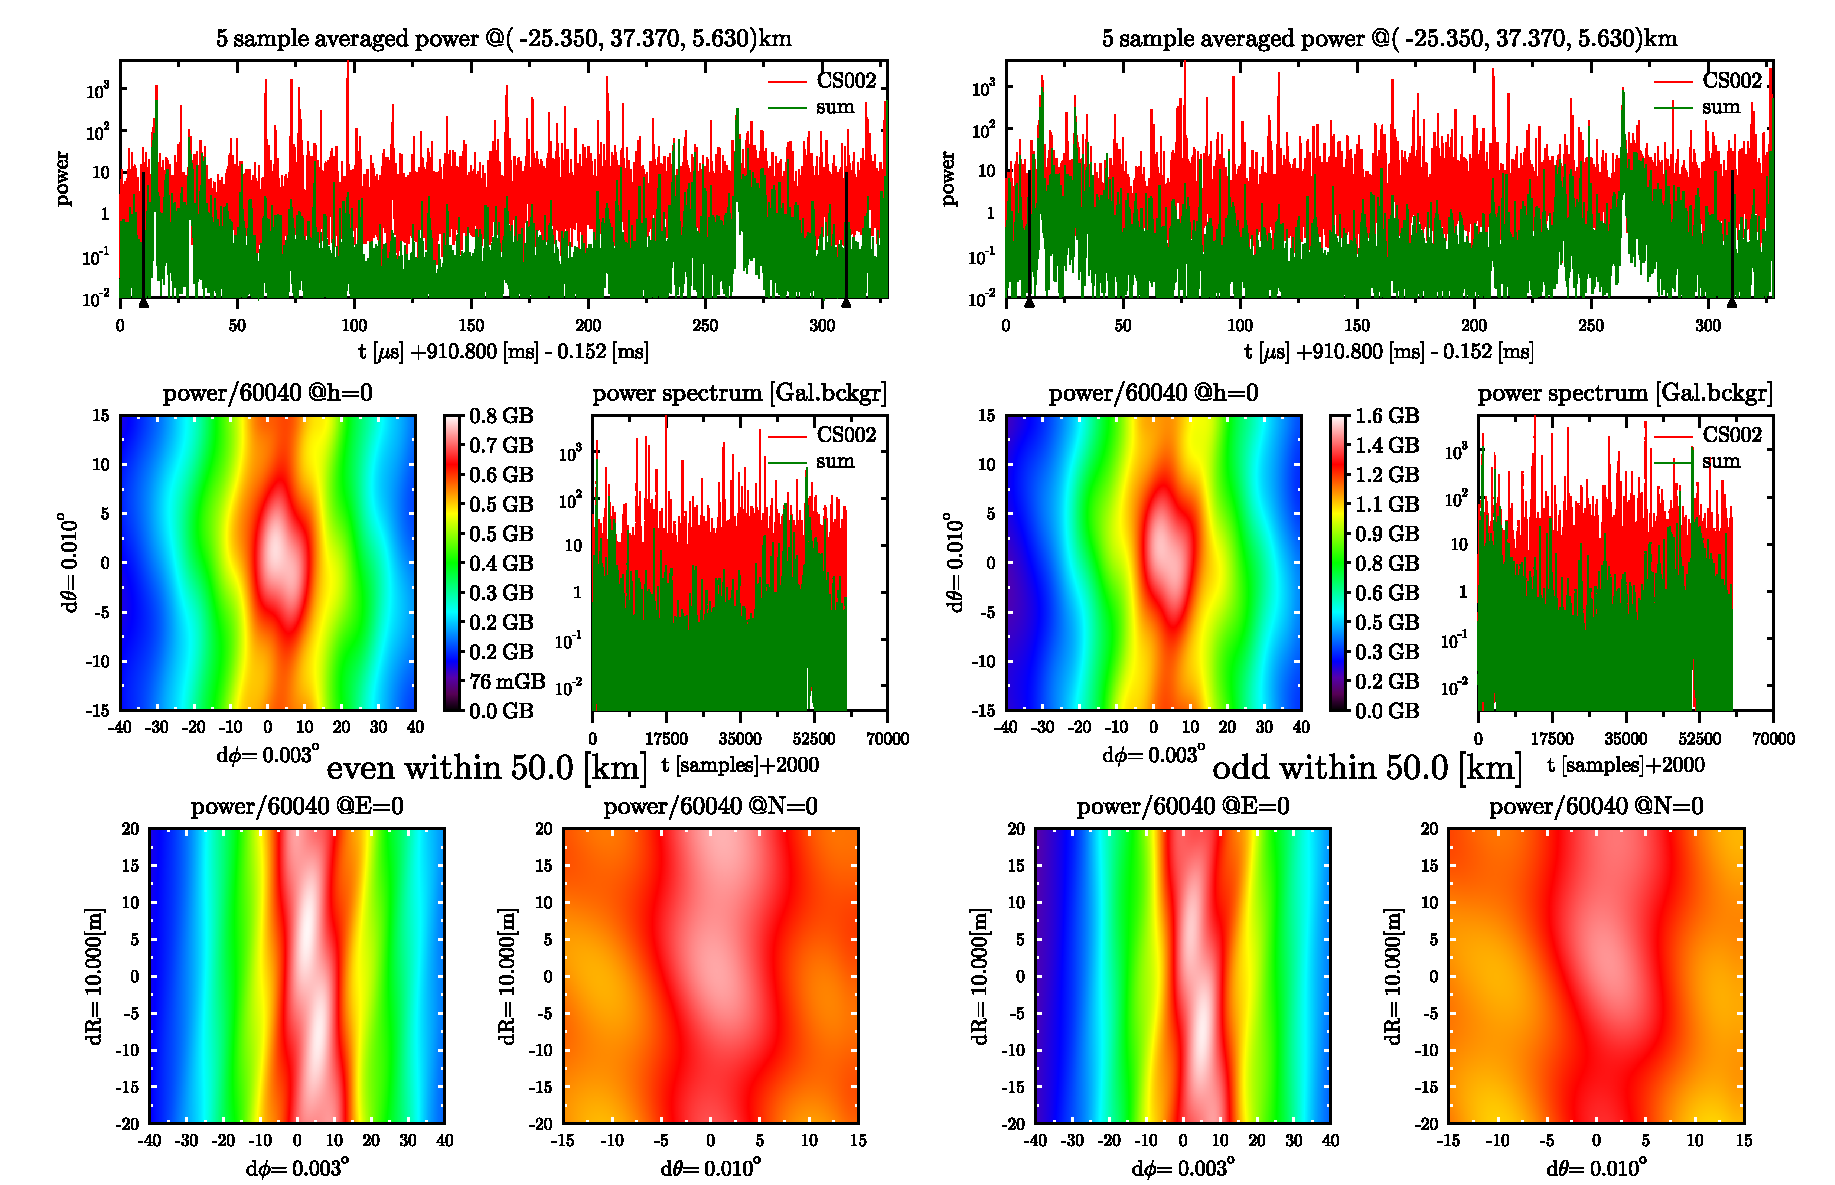
\includegraphics[width=0.99\textwidth]{Figs/InterfContourSE20A7-Np-} }
%\centering{\includegraphics[ bb=1.0cm 2.4cm 24.5cm 25.7cm,clip, width=0.49\textwidth]{../Figs/SE20A7-NPMx_1HIntfSpecSel} }
	\caption{Typical beamforming-intensity plot (name starting with `EIContour') as generated by running the TRI-D Imager.}	 \figlab{TRIDIntImg}
\end{figure}

A typical interferometric Intensity plot is shown in \figref{TRIDIntImg}. The data used for producing this plot are not saved.
\\Top panel: The time trace for the complete chunk of data in the reference antenna for the two dipoles. The selected time window for TRI-D imaging is indicated by the black triangles. For the case of \figref{TRIDIntImg} [line +3] reads `\verb!F   2000   1995 10.000 !' implying that the time window starts lies between sample 2000 or 10~$\mu$s and sample 3995 or about 20~$\mu$s. The time offset is written as the offset in the reference antenna plus the time difference with that at the center voxel.
\\middle left panel: The beamforming-intensity for the voxels at the central height. The axes in this plot give Easying and Northing with respect to the central voxel and the voxel size is shown on the axes. The intensity is integrated over the complete time window, listed on top of this panel.
\\middle central panel: The beamforming-intensity time trace for the central voxel summing the transverse (1+2) polarizations as seen from the core.
\\middle right panel: Showing (for the central voxel) the time trace for the transverse Stokes parameters, Q, U, V, normalized by the intensity. For a time trace with much background this plot is messy.
\\bottom left \& right panels: same as middle left panel for different cuts through the image cube.

\subsubsection{TRI-D Source position plot}\seclab{TRID-locate}

\begin{figure}[th]
\setlength{\unitlength}{.49\textwidth} % .43\textwidth}
   \subfloat[`IntfMx\_']{ \centering{\includegraphics[width=0.43\textwidth]{Figs/IntfMx_db-D3+05} } \figlab{TRIDSrcsImg}}
   \subfloat[`IntfPol\_']{ \centering{\includegraphics[bb=0.0cm 0cm 23cm 39cm,clip,width=0.43\textwidth]{Figs/IntfPol_db-D3+05} } \figlab{TRIDPolImg} }
%\centering{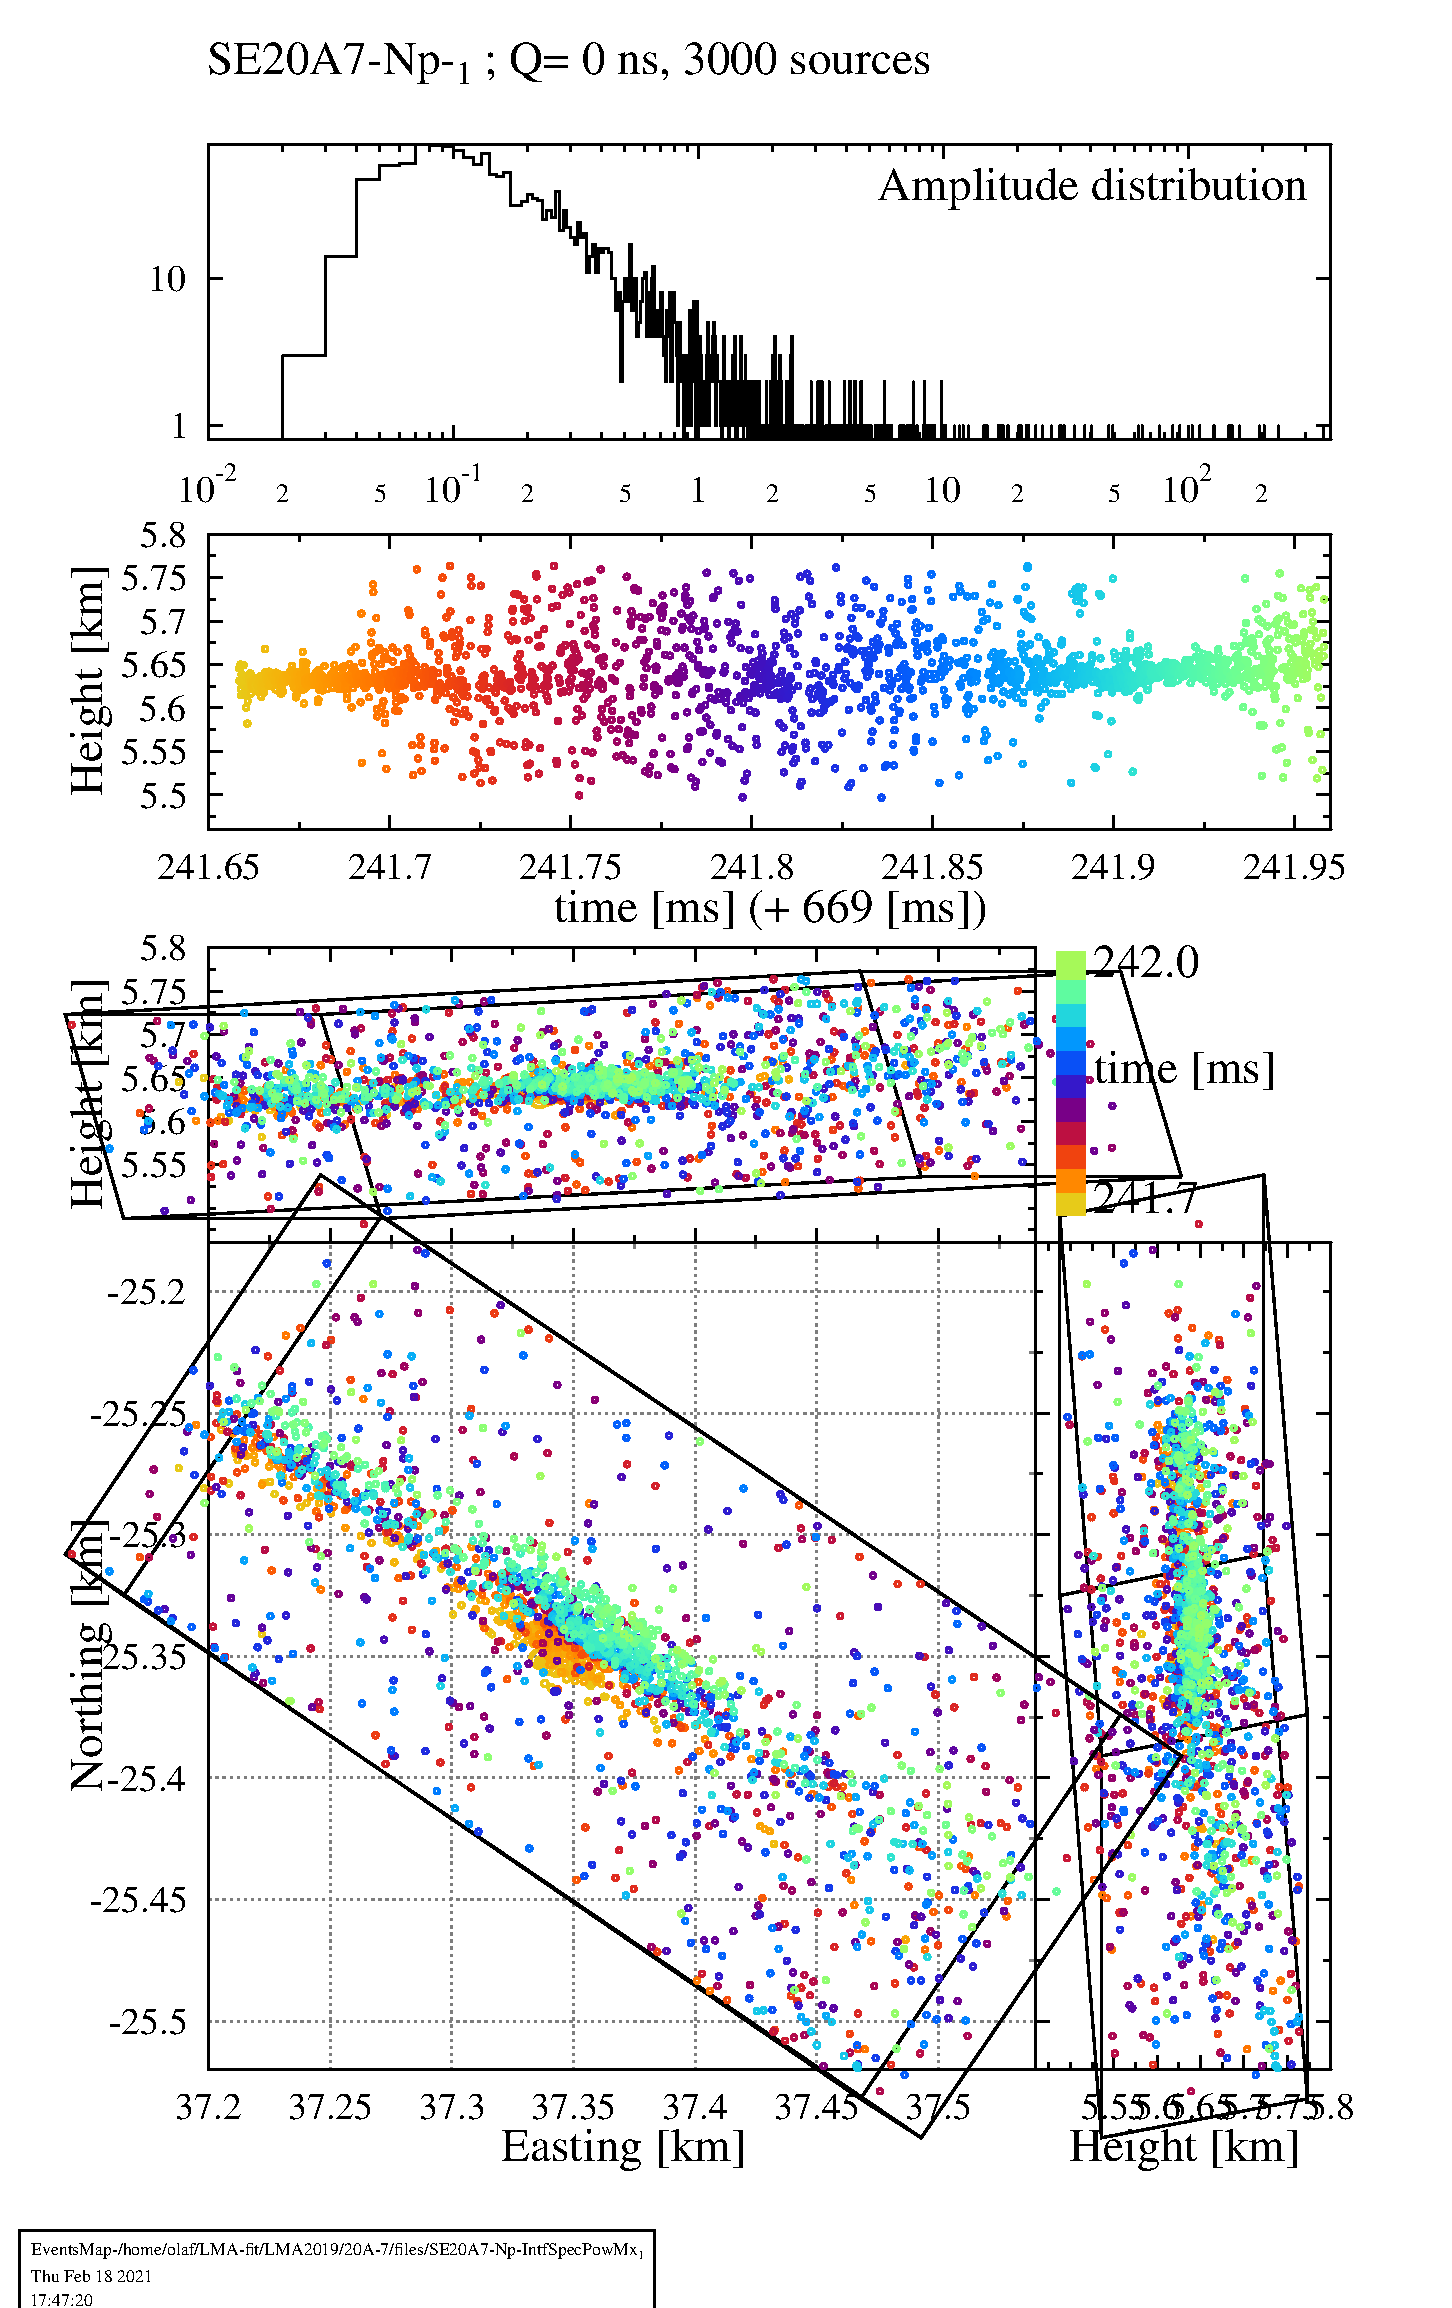
\includegraphics[width=0.49\textwidth]{Figs/SE20A7-Np--InfImaMx_1} }
%\centering{\includegraphics[ bb=1.0cm 2.4cm 24.5cm 25.7cm,clip, width=0.49\textwidth]{../Figs/SE20A7-NPMx_1HIntfSpecSel} }
	\caption{Plots generated by running the TRI-D imager where \figref{TRIDSrcsImg} shows a typical beamforming image plot (name starting with `IntfMx\_') and \figref{TRIDPolImg} a typical source polarization plot (name starting with `IntfPol\_').}	
\end{figure}

The located sources are given in \figref{TRIDSrcsImg} as well as the hypercube that was used for imaging. Sources close to the borders of this hypercube should not be trusted. The size of the wagon-wheels are a proxy for the relative intensities of the sources, where the size for the largest wagon-wheel is set by the 4$^{th}$ parameter on [line +3]. If negative, only dots are plotted and also the intensity plot (top panel) will be omitted.

The interferometric hypercube is also shown.

\subsubsection{TRI-D Source polarization plot}

A quick overview is presented of a variety of source-polarization observables. All are listed for each slice where the source obeyed the imaging conditions (not too close to the edge of the image cube, intensity above some threshold).
\\Top or 7$^{th}$ panel: the percentages of the linear, circular and unpolarized intensity.
\\6$^{th}$ panel: The $\chi^2$ of the fit to the time traces in all antennas for this slice. The $\chi^2$ tends to be large for strong peaks, implying that the error estimates on the trace amplitudes is not well under control and needs further scrutiny.
\\5$^{th}$ panel: The ratio of the intensity in the longitudinal (I3, as seen from the reference) direction compared to the total beamforming intensity as reconstructed by the imager. This ratio tends to be large for poorly reconstructed sources.
\\4$^{th}$ \& 3$^{rd}$ panels: The angular orientation of the dipole density per slice. For each slice a principal component analysis (PCA) is performed of the polarization directions per sample in the slice. Shown are the directions of the main (in red) and that of the secondary axes (in green) of the distribution. The error bars denote the amount of circular polarization. This is given as an error bar as one would expect that for a very long time trace the circular polarization should average to zero as there is -physics wise, because of symmetries- no reason for a net circular polarization. For short time traces the circular polarization will be non-zero due to random fluctuations. Note that the three axes are perpendicular.
\\2$^{nd}$ panel: Length of the three axes (red, green and yellow) if they are above a certain threshold.
\\bottom panel: The red line shows the summed transverse intensity for the reference antenna. The magenta dots give the transverse intensity for the slice at the source location. This should always be larger than that for the reference station in the default imaging conditions are used. The black dots show the total intensity, transverse + longitudinal, for the source.

\subsection{Selective plotting}\seclab{InterfSrcSel}

Note: This section in obsolete by now since the utility "InterfSrcSel" is superseded by "DataSelect" discussed in \secref{DataSelect}.

\Omit{ -------------------------------------------------------------
The script \verb!"InterfSrcSel.sh"! using \verb!"InterfSrcSel.in"! as input allows to produce plots that are zoomed in on the region of interest. This script plots the position of the sources using the GLE-script, \verb!"SourcesPlot.gle"! and the distribution of sources intensities using \verb!"SourcesPlot.gle"!. These are run via spawned scripts on Windows as well as Linux machines.
A typical input resembles:

\begin{linenumbers}
\resetlinenumber
\begin{verbatim}
&Parameters
 OutFileLabel="XYZ",     ! Normal Negative Leader (a)
 DataFile=   "SE20A7-Nh-", "SE20A7-Nh:-10", "SE20A7-Nh:-09", "SE20A7-Nh:-08", "SE20A7-Nh:-07", "SE20A7-Nh:-06"
   "SE20A7-Nh:-05"
 SMPowCut = 3.,       ! power of pulse included in the plot
 AmpltPlot=0.1       !  dependence of dot sizes on pulse power
 MaxAmplFitPercent=0.001      ! Maximal percentile amplitudes to be included in fits of power-spectrum
 ZoomClip = .true.   ! clip sources outside plotting region
 xmin=37.15 , xmax=37.6, ymin=-25.45, ymax=-25.15, zmin=5.35, zmax=5.8,  tmin=237.0 , tmax=245.3
&End
\end{verbatim}
\end{linenumbers}

The lines in the namelist \verb!"&Parameters"! input specify:
\begin{enumerate}
\item[2] \verb!"OutFileLabel="!: Additional label used for the output files, including the plots.
\item[3] \verb!"DataFile="!: Distinctive \verb!"XYZ"! labels of the data files discussed in \secref{InterfSrc}. The data of all these files will be sorted in time and used for plotting and producing the intensity distributions.
\item[5] \verb!"SMPowCut="!: Only stronger sources are used for plotting.
\item[6] \verb!"AmpltPlot="!: A factor used for scaling the dot-size when plotting. If zero all dots are the same size.
\item[7] \verb!"MaxAmplFitPercent="!: Percentile cut for the sources included in fitting a power-law to the distribution. Stronger sources are excluded.
\item[8] \verb!"ZoomClip="!: Clip source locations to the plotting volume.
\item[9] \verb!"xmin="!: The bounding boxes used in space and time for the plots.
\end{enumerate}

\begin{figure}[th]
\centering{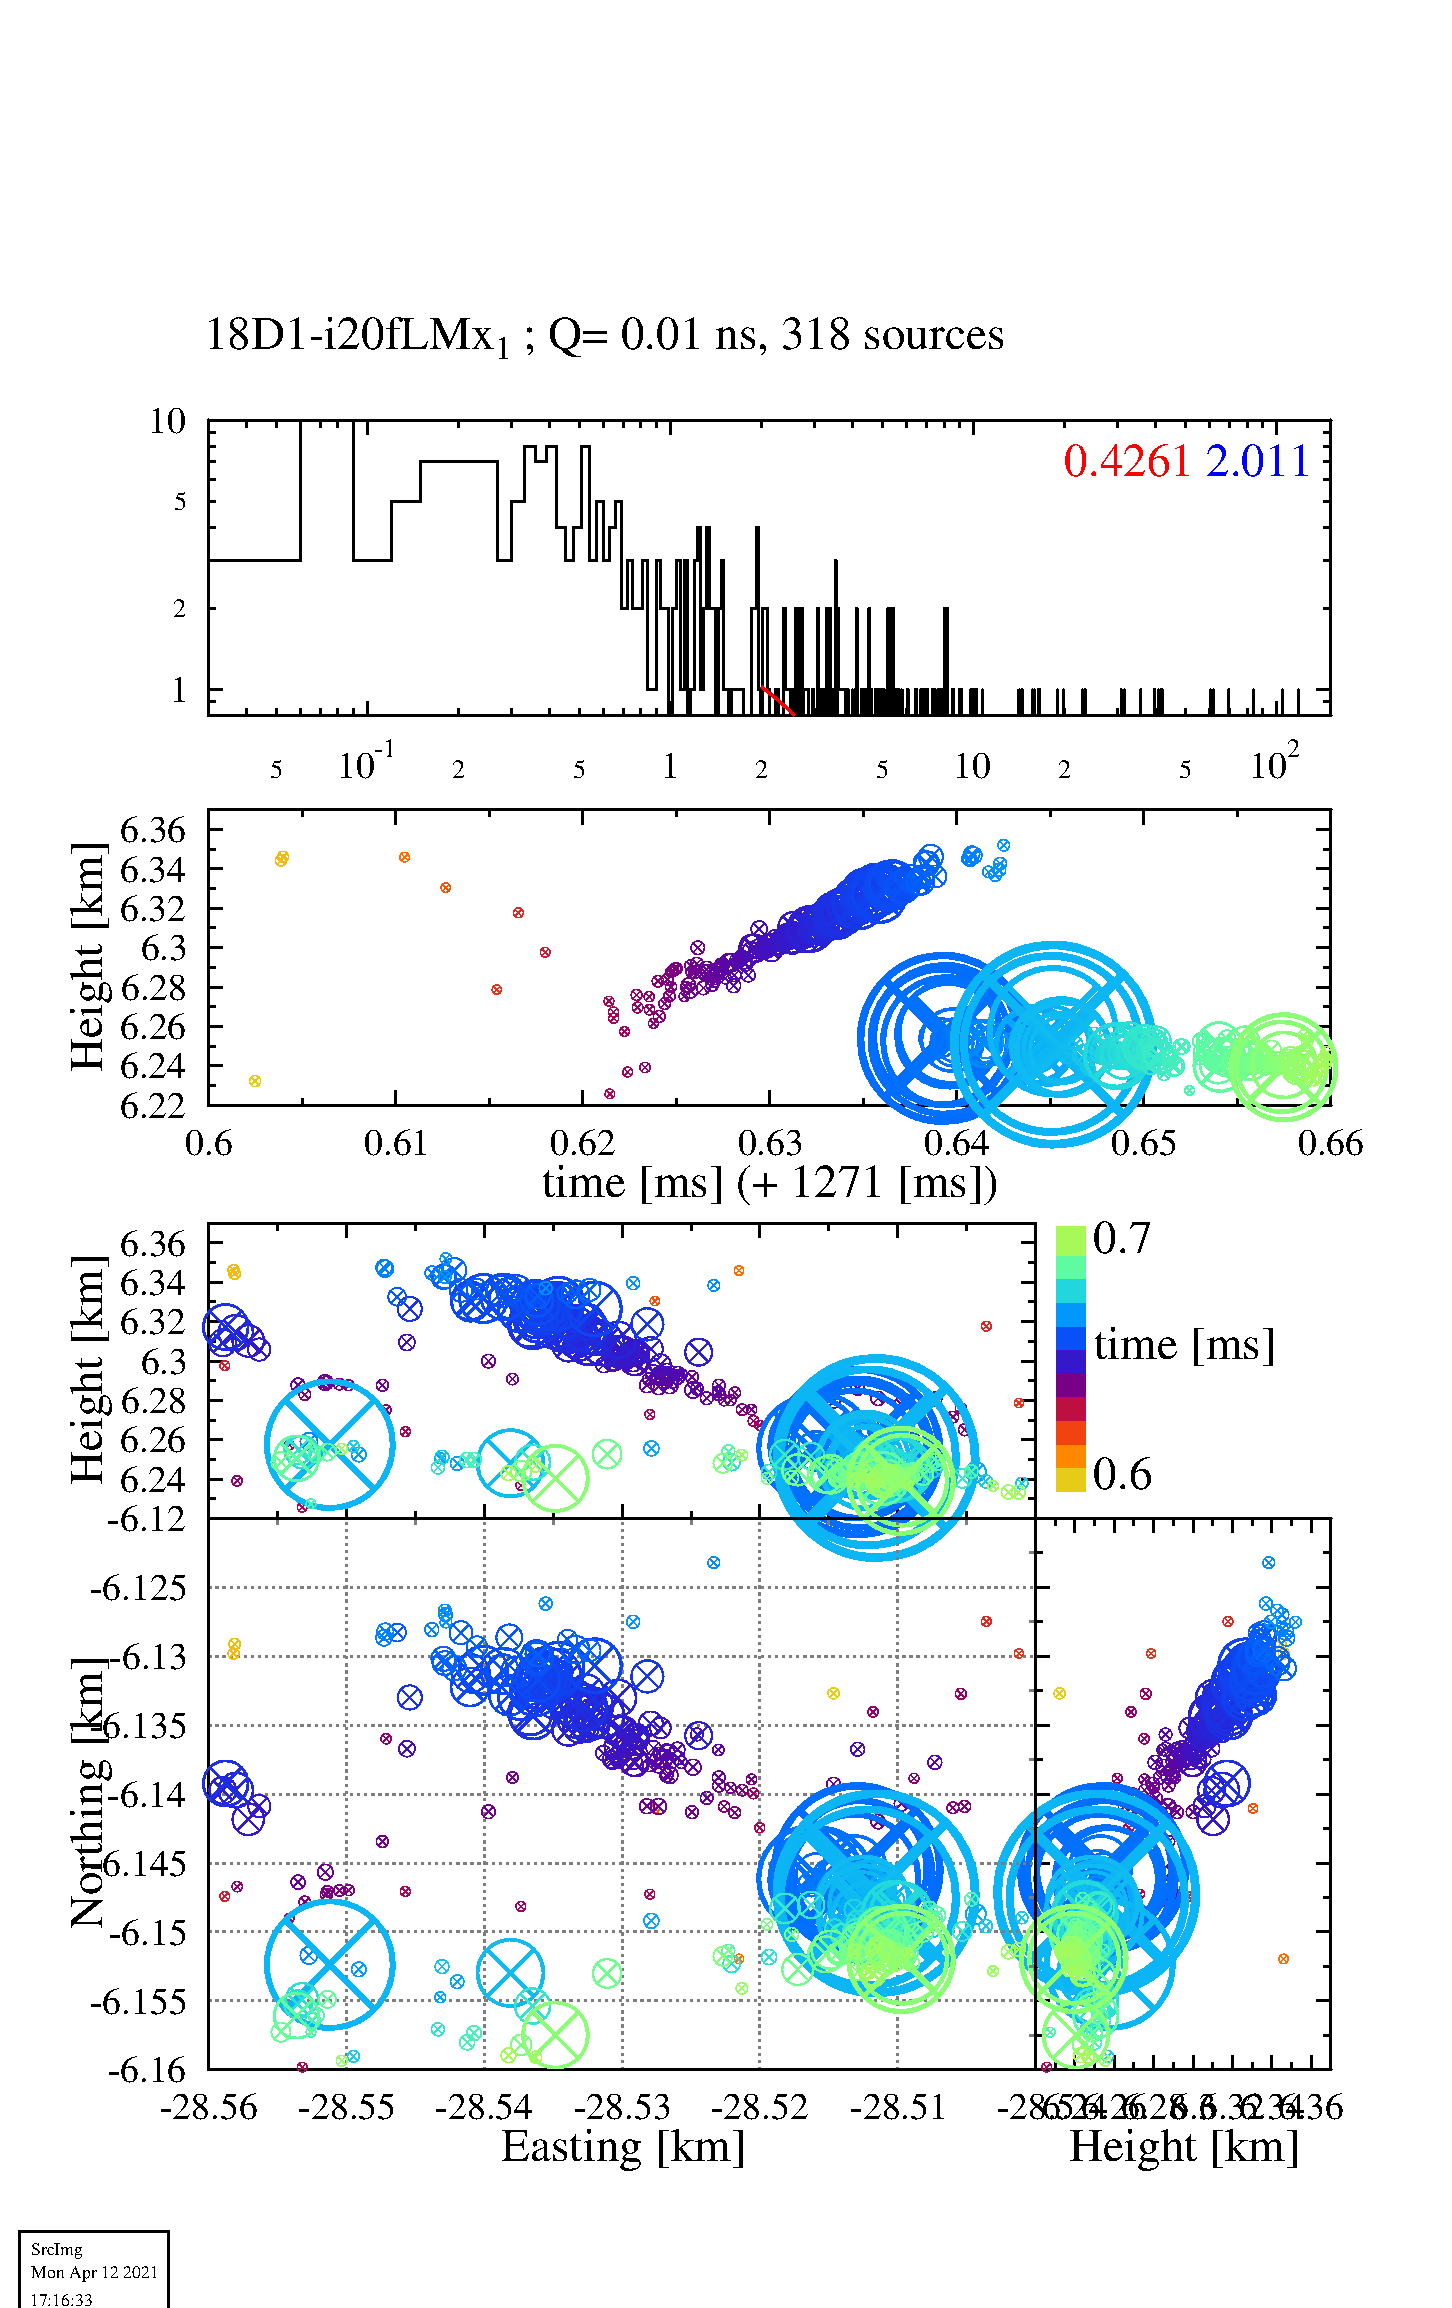
\includegraphics[width=0.49\textwidth]{Figs/18D1-i20fMx_1LIntfSpecSel} }
%\centering{\includegraphics[ bb=1.0cm 2.4cm 24.5cm 25.7cm,clip, width=0.49\textwidth]{../Figs/SE20A7-NPMx_1HIntfSpecSel} }
	\caption{Typical image for the TRID Imager as created by running ``InterfSrcSel.sh".}	 \figlab{TRIDSelSrcsImg}
\end{figure}

The plots will be made for the `Mx' and `Bar' files as well as for X- and Y-dipoles, all resembling \figref{TRIDSelSrcsImg}. This allows for appending seamless the results of different interferometry runs.

} %---------------------------------------------------------------------
